Artifact sharing and reproducible experimentation are key
for our collaborative approach to machine-learning based optimization
and co-design of computer systems, which was first prototyped
during the EU-funded MILEPOST project~\cite{Fur2009,milepost,29db2248aba45e59:a31e374796869125}.
%
Indeed, it is difficult, if not impossible, and time consuming to build useful predictive models
without large and diverse training sets (programs, data sets),
and without crowdsourcing design and optimization space exploration
across diverse hardware~\cite{new_pub_model,cm:29db2248aba45e59:cd11e3a188574d80}.%

While we have been actively promoting artifact sharing for the past 10 years
since the MILEPOST project~\cite{Fur2009,ctuning1}, it is still relatively rare in the community
systems community.
%
We have begun to understand possible reasons for that through our Artifact
Evaluation initiative~\cite{ctuning-ae1,childers2016artifact} 
at PPoPP, CGO, PACT, SuperComputing and other leading ACM and IEEE conferences
which has attracted over a hundred of artifacts in the past few years.

   %%%%%%%%%%%%%%%%%%%%%%%%%%%%%%%%%%%%%%%%%%%%%%%%%%%%%%%%%%%%%%%%%%%%%%%%%%%%%%%%%%%%%%%%%
   %CK={"action":"prepare_for_latex", "cid":"slide:678dbc30be21a7ab", "file":"4094a9fad1c48a5e-cropped.pdf", "path":"ck-assets", "ck_image":"yes", "ck_image_width":900}
   \begin{figure*}[htbp]
     \centering
      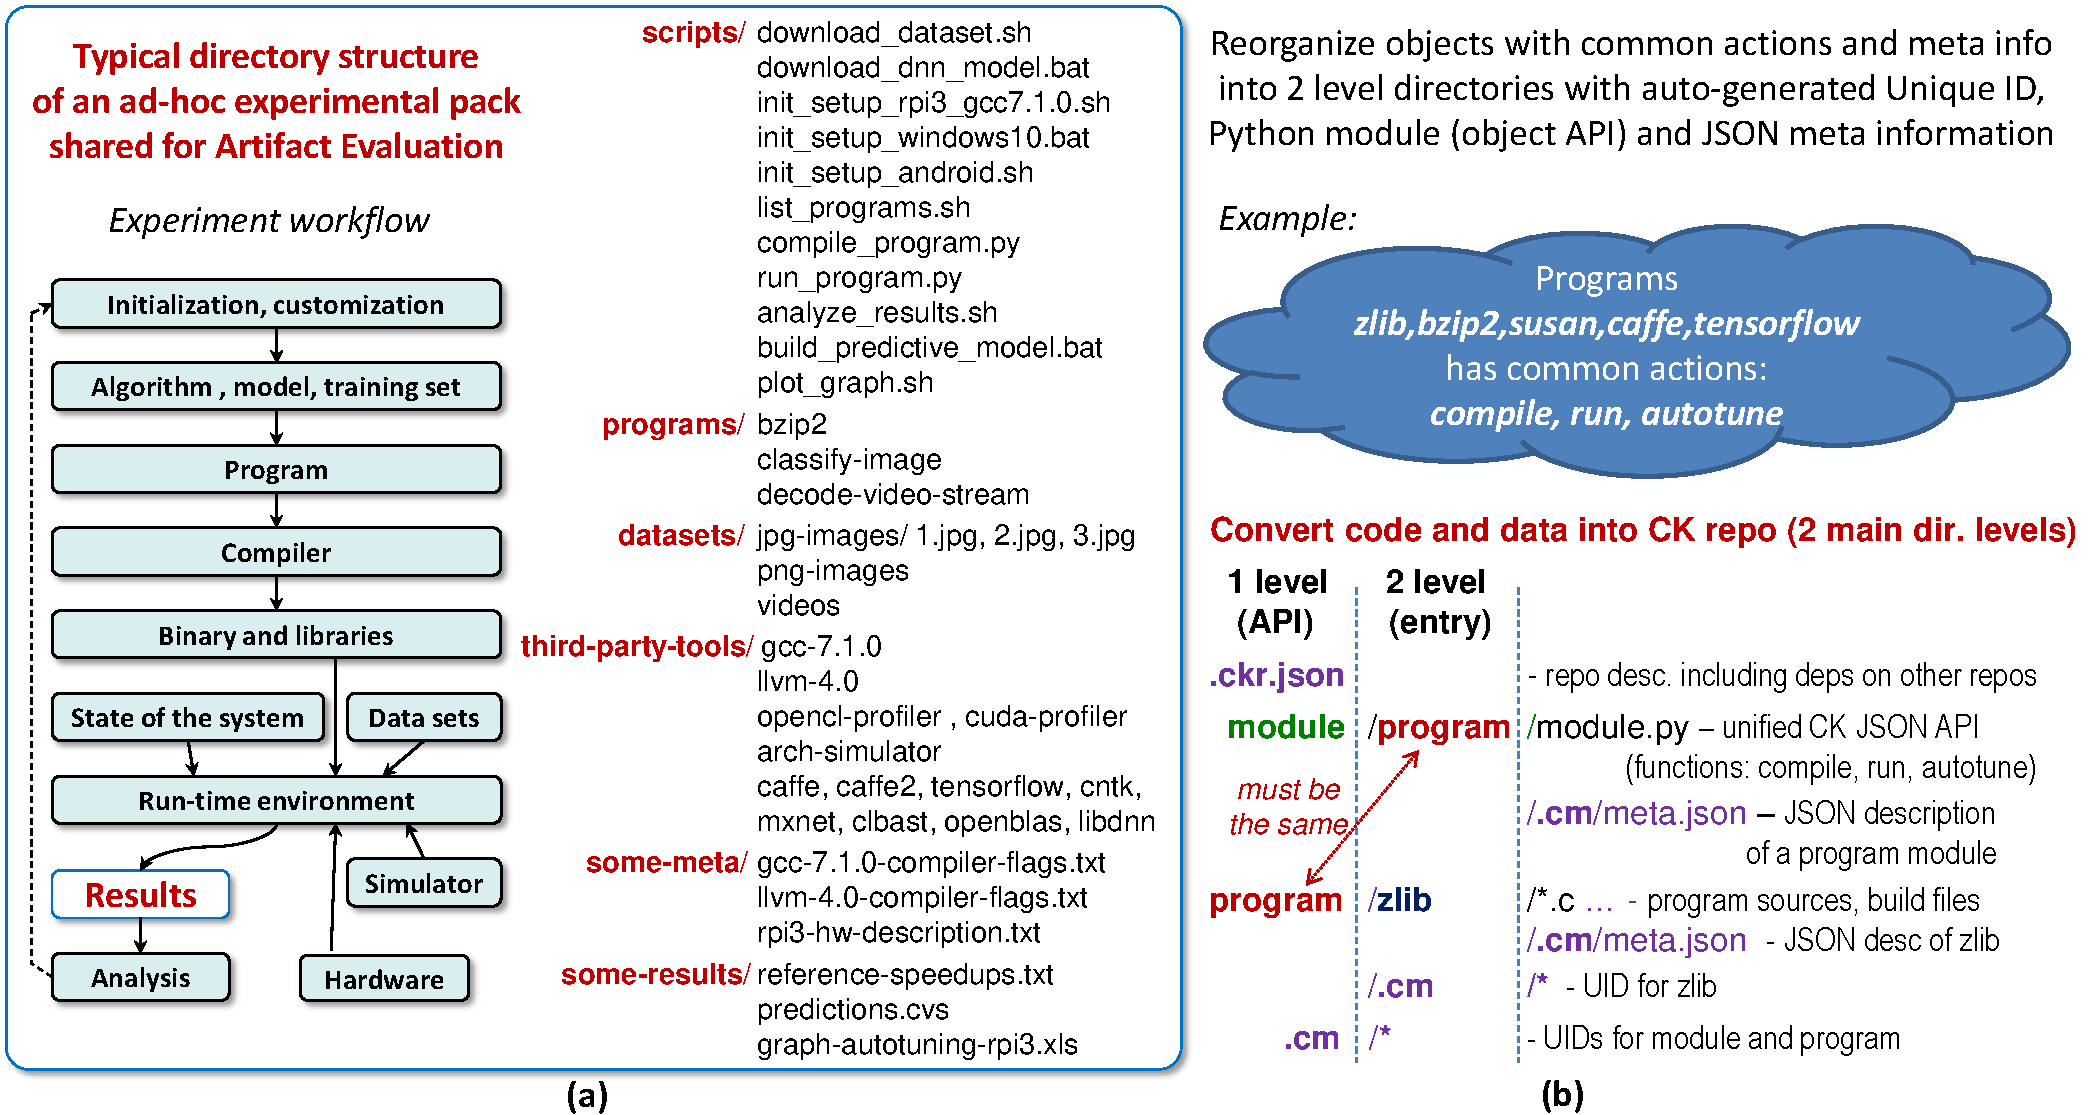
\includegraphics[width=6.5in]
      {ck-assets/4094a9fad1c48a5e-cropped.pdf} %CK_URL={4094a9fad1c48a5e-cropped.pdf}
     \caption{
       Reorganizing ad-hoc experimental packs into reusable, customizable and discoverable components
       with JSON API and meta information using the Collective Knowledge framework.
     }
     \label{fig:convert-to-ck}
   \end{figure*}
   %%%%%%%%%%%%%%%%%%%%%%%%%%%%%%%%%%%%%%%%%%%%%%%%%%%%%%%%%%%%%%%%%%%%%%%%%%%%%%%%%%%%%%%%%

Unfortunately, nearly all the artifacts have been shared simply as zip
archives, GitHub/GitLab/Bitbucket repositories, or VM/Docker images, with many
ad-hoc scripts to prepare, run and visualize experiments, as shown in
Figure~\ref{fig:convert-to-ck}a.
%
While a good step towards reproducibility, such ad-hoc artifacts are hard to
reuse and customize as they do not provide a common API and meta information.

Some popular and useful services such as Zenodo~\cite{zenodo} and
FigShare~\cite{figshare} allow researchers to upload individual artifacts to
specific websites while assigning DOI~\cite{doi} and providing some meta
information.
%
This helps the community to discover the artifacts, but does not necessarily
make them easy to reuse.

After an ACM workshop on reproducible research methodologies (TRUST'14)~\cite{trust2014}
and a Dagstuhl Perspective workshop on Artifact Evaluation~\cite{childers2016artifact},
we concluded that compute systems research lacked a common experimental
framework in contrast with other sciences~\cite{doi:10.1093/bioinformatics/bth361}.

Together with our fellow researchers, we also assembled the following wish-list
for such a framework:

\begin{itemize}

\item it should be able to help researchers quickly organize their local code
and data into discoverable and reusable components with a unique ID, common API
and unified meta information, rather than being forced to upload them to the
web from the start;

\item it should be open-source with a permissive license to simplify technology
transfer;

\item it should be portable, simple to install and use from the command line;

\item it should allow to assemble experimental workflows by simply plugging in
shared components;

\item it should support native non-virtualized execution of such workflows,
i.e.\ not only via Virtual Machine~\cite{Smith:2005:AVM:1069588.1069632} and
Docker~\cite{docker}, critical for empirical program optimization and hardware
co-design experiments;

\item it should be able to adapt to continuously evolving software environments
and support different versions of tools such as rapidly evolving
compilers and libraries;

\item it should include a local web server to simplify crowdsourcing of
experiments and visualization of results in workgroups.

\end{itemize}

Since there was no available open-source framework with all these features,
we decided to develop such a framework, Collective Knowledge (CK)~\cite{ck,ck-date16}, 
from scratch with initial support from the EU-funded TETRACOM project~\cite{tetracom}.
%
CK is implemented as a small and portable Python module with a command line
front-end to assist users in converting their local objects (code and data)
into searchable, reusable and shareable directory entries with user-friendly
aliases and auto-generated Unique ID, JSON API and JSON meta
information~\cite{json-org}, as described in~\cite{ck-date16,ck-concepts} and 
conceptually shown in Figure~\ref{fig:convert-to-ck}b.

The user first creates a new local CK repository as follows:
\begin{flushleft}
\texttt{\$ ck add repo:new-ck-repo}
\end{flushleft}

Initially, it is just an empty directory:
\begin{flushleft}
\texttt{\$ ck find repo:new-ck-repo} \newline
\texttt{\$ ls `ck find repo:new-ck-repo`}
\end{flushleft}

Now, the user starts adding research artifacts as CK components with extensible APIs.
%
For example, after noticing that we always perform 3 common actions on all our benchmarks
during our experiments, "compile", "run" and "autotune", we want to provide a common
API for these actions and benchmarks, rather than writing ad-hoc scripts.
%
The user can provide such an API with actions by adding a new CK module to a CK repository as follows:
\begin{flushleft}
\texttt{\$ ck add new-ck-repo:module:program}
\end{flushleft}
%
CK will then create two levels of directories \textit{module} and \textit{program} in the \textit{new-ck-repo}
and will add a dummy \textit{module.py} where common object actions can be implemented later.
%
CK will also create a sub-directory \textit{.cm} (collective meta) 
with an automatically generated Unique ID of this module and various pre-defined 
descriptions in JSON format (date and time of module creation, author, license, etc)
to document provenance of the CK artifacts.

Users can now create holders (directories) for such objects sharing common CK module and an API as follows:
\begin{flushleft}
\texttt{\$ ck add new-ck-repo:program:new-benchmark}
\end{flushleft}
%
CK will again create two levels of directories: 
the first one specifying used CK module (\textit{program}) 
and the second one with alias \textit{new-benchmark} 
to keep objects.
%
CK will also create three files in an internal \textit{.cm} directory:

\begin{itemize}

\item \textbf{meta.json} - an empty JSON file which can be gradually extended 
to describe a given object (such as added program in our example);

\item \textbf{info.json} - a JSON file with the date and time of the last modification
as well as license, copyright and author information to keep attribution of all updates
for open research;

\item \textbf{desc.json} - an empty JSON file to describe types of keys in \textbf{meta.json}
(useful for automatic type checking) and their value ranges (useful for autotuning
as we will show later in this report).

\end{itemize}

%
Users can then find a path to a newly created object holder (CK entry) using
the \textit{ck find program:new-benchmark} command and then copy all files and
sub-directories related to the given object using standard OS shell commands.

   %%%%%%%%%%%%%%%%%%%%%%%%%%%%%%%%%%%%%%%%%%%%%%%%%%%%%%%%%%%%%%%%%%%%%%%%%%%%%%%%%%%%%%%%%
   %CK={"action":"prepare_for_latex", "cid":"slide:678dbc30be21a7ab", "file":"bb46e3bcbfa20c5f-cropped.pdf", "path":"ck-assets", "ck_image":"yes", "ck_image_width":750}
   \begin{figure*}[htbp]
     \centering
      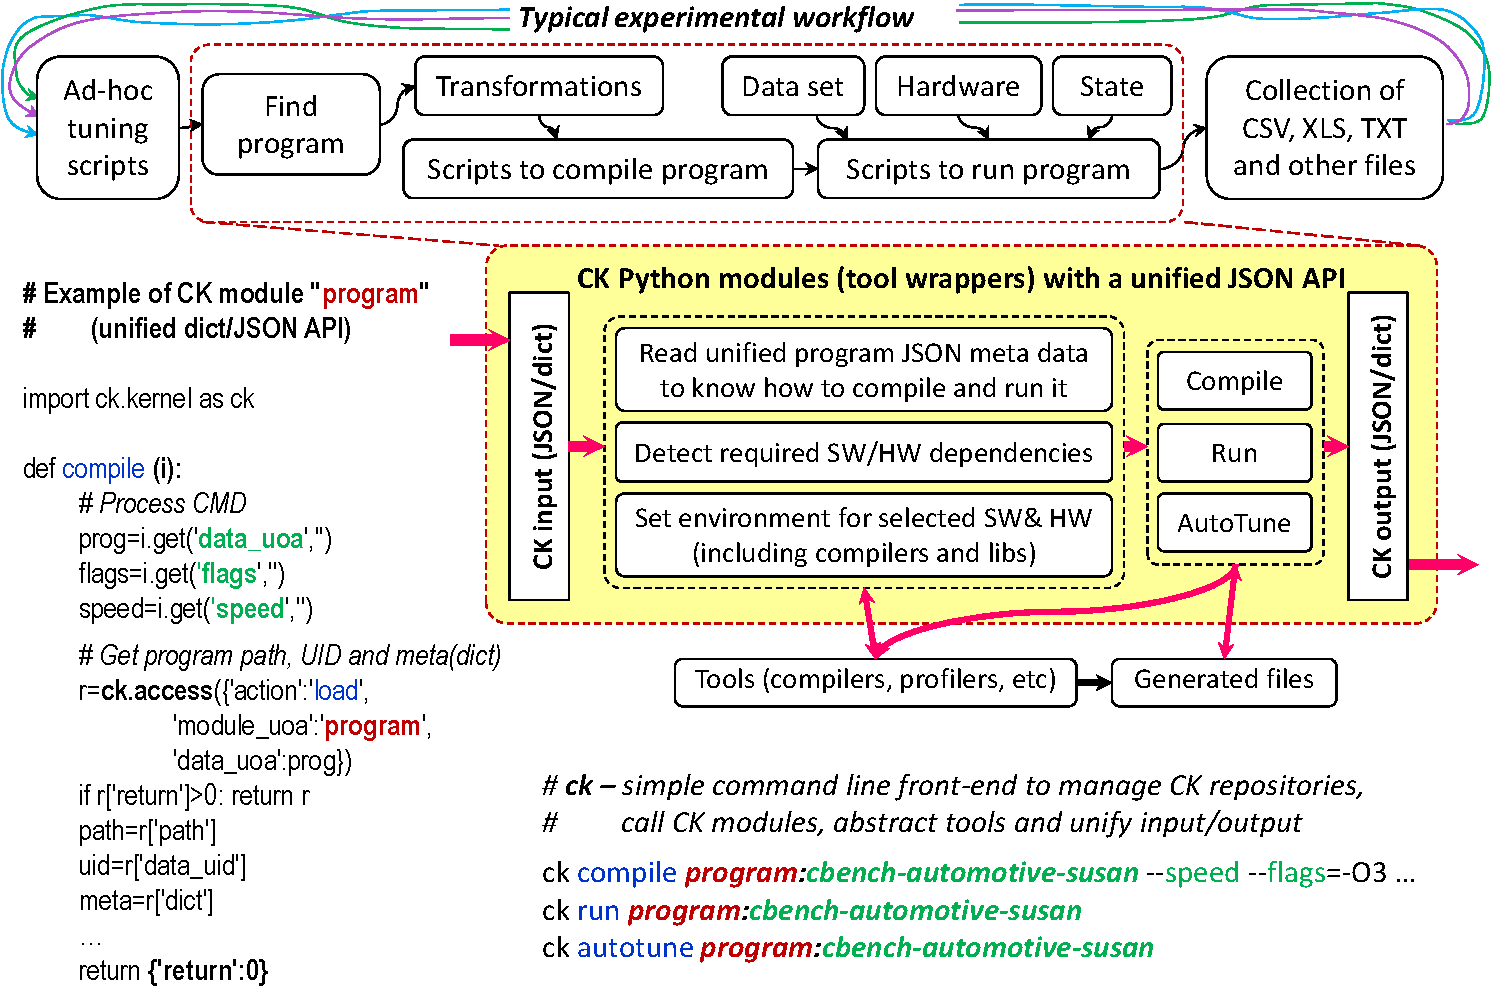
\includegraphics[width=6in]
      {ck-assets/bb46e3bcbfa20c5f-cropped.pdf} %CK_URL={bb46e3bcbfa20c5f-cropped.pdf}
     \caption{
        Converting ad-hoc scripts, tools and workflows to CK Python modules
        and standardized directories with actions, unified JSON API, and JSON meta information.
     }
     \label{fig:ck-workflows}
   \end{figure*}
   %%%%%%%%%%%%%%%%%%%%%%%%%%%%%%%%%%%%%%%%%%%%%%%%%%%%%%%%%%%%%%%%%%%%%%%%%%%%%%%%%%%%%%%%%

This allows to get rid of ad-hoc scripts by implementing actions inside
reusable CK Python modules as shown in Figure~\ref{fig:ck-workflows}.
%
For example, the user can add an action to a given module such as \textit{compile program}
as follows:
\begin{flushleft}
\texttt{\$ ck add\_action module:program --func=compile}
\end{flushleft}
%
CK will create a dummy function body with an input dictionary \textit{i}
inside \textit{module.py} in the CK \textit{module:program} entry.
%
Whenever this function is invoked via CK using the following format:
\begin{flushleft}
\texttt{\$ ck compile program:some\_entry --param1=val1}
\end{flushleft}
the command line will be converted to \textit{i} dictionary
and printed to the console to help novice users understand the CK API.
%
The user can now substitute this dummy function with a specific action on a specific entry
(some program in our example based on its meta information)
as conceptually shown in Figure~\ref{fig:ck-workflows}.
%
The above example shows how to call CK functions from Python modules rather than from the command line
using the \textit{ck.access} function.
%
It also demonstrates how to find a path to a given \textit{program} entry,
load its meta information and unique ID.
%
For the reader's convenience, Figure~\ref{fig:ck-commands} lists several important CK commands.

   %%%%%%%%%%%%%%%%%%%%%%%%%%%%%%%%%%%%%%%%%%%%%%%%%%%%%%%%%%%%%%%%%%%%%%%%%%%%%%%%%%%%%%%%%
   %CK={"action":"prepare_for_latex", "cid":"slide:678dbc30be21a7ab", "file":"ef7349a78679ca71-cropped.pdf", "path":"ck-assets", "ck_image":"yes", "ck_image_width":600}
   \begin{figure*}[htbp]
     \centering
      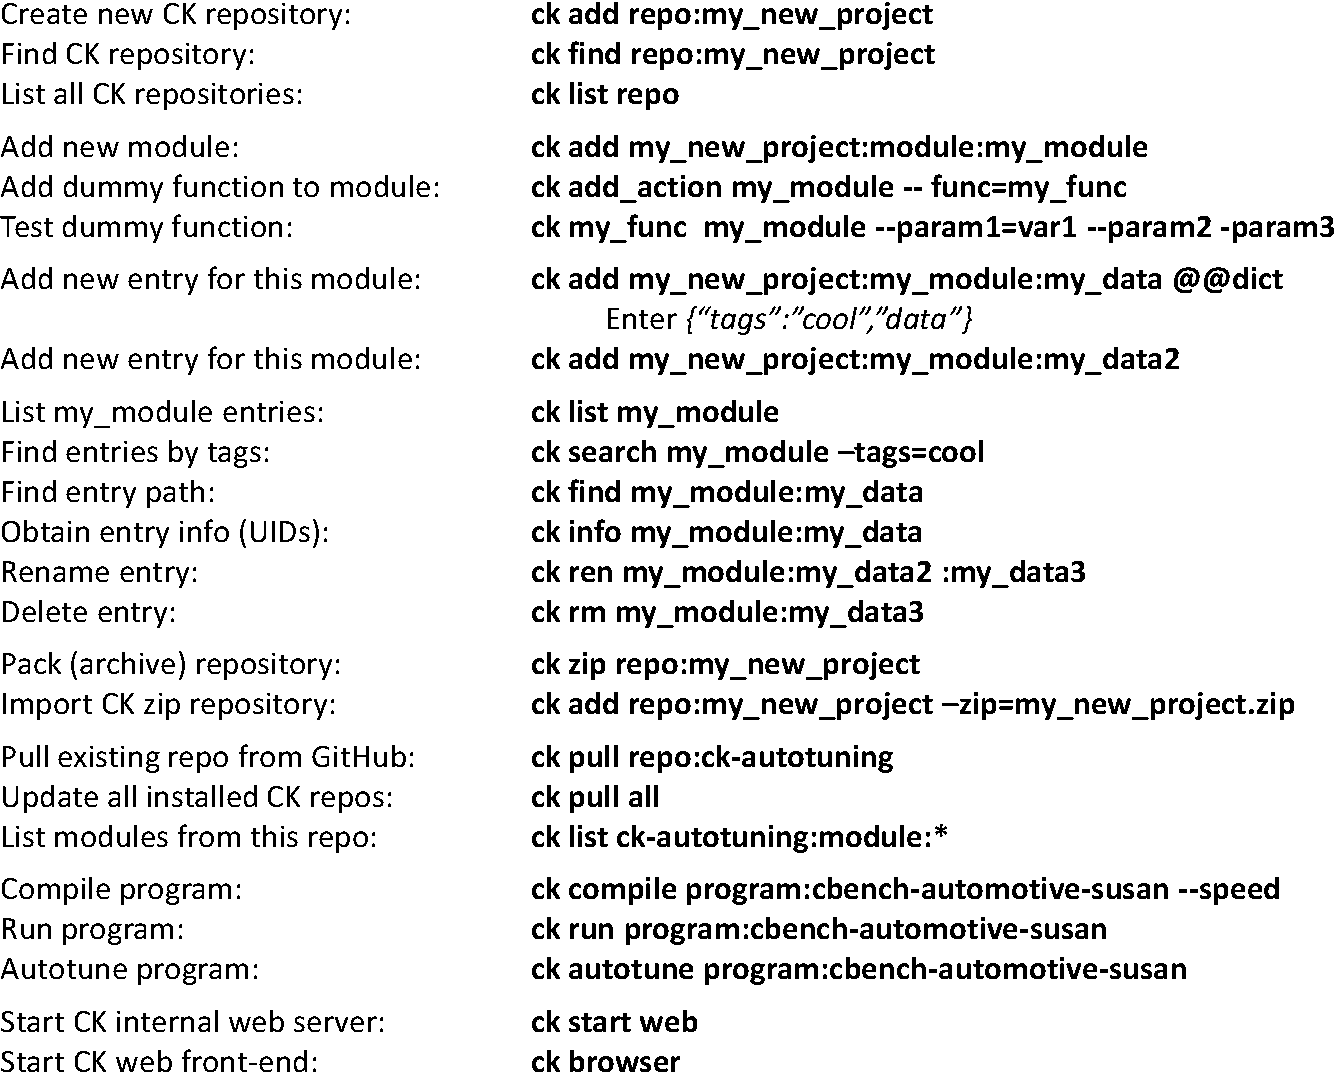
\includegraphics[width=4.8in]
      {ck-assets/ef7349a78679ca71-cropped.pdf} %CK_URL={ef7349a78679ca71-cropped.pdf}
     \caption{
        Main CK commands to create new or pull existing repositories, add modules, manage entries, perform actions, and use a local web server.
     }
     \label{fig:ck-commands}
   \end{figure*}
   %%%%%%%%%%%%%%%%%%%%%%%%%%%%%%%%%%%%%%%%%%%%%%%%%%%%%%%%%%%%%%%%%%%%%%%%%%%%%%%%%%%%%%%%%

This functionality should be enough to start implementing unified compilation and execution
of shared programs.
%
For example, the \textit{program} module can read instructions about how to compile and run
a given program from the JSON meta data of related entries, prepare and execute portable sub-scripts,
collect various statistics, and embed them to the output dictionary in a unified way.
%
This can be also gradually extended to include extra tools into compilation and execution workflow
such as code instrumentation and profiling.

Here we immediately face another problem common for computer systems research:
how to support multiple versions of various and continuously evolving tools and libraries?
%
However, since we no longer hardwire calls to specific tools directly in scripts
but invoke them from higher-level CK modules, we can detect all required tools
and set up their environment before execution.
%
To support this concept even better, we have developed a cross-platform package manager
as a \href{https://github.com/ctuning/ck-env}{ck-env} repository~\cite{ck-env} with several CK modules
including \textit{soft}, \textit{env}, \textit{package}, \textit{os} and \textit{platform}.
%
These modules allow the community to describe various operating systems (Linux, Windows, MacOS, Android);
detect platform features (\textit{ck detect platform}); detect multiple-versions of
already installed software (\textit{ck detect soft:compiler.gcc});
prepare CK entries with their environments for a given OS and platform
using \textit{env} module (\textit{ck show env}) thus allowing easy co-existence of multiple versions of a given tool;
install missing software using \textit{package} modules;
describe software dependencies using simple tags
in a program meta description (such as \textit{compiler,gcc} or \textit{lib,caffe}),
and ask the user to select an appropriate version during program compilation when multiple software
versions are registered in the CK as shown in Figure~\ref{fig:portable-package-manager}.

   %%%%%%%%%%%%%%%%%%%%%%%%%%%%%%%%%%%%%%%%%%%%%%%%%%%%%%%%%%%%%%%%%%%%%%%%%%%%%%%%%%%%%%%%%
   %CK={"action":"prepare_for_latex", "cid":"slide:70cad42254c3bb15", "file":"01714ac89d5bd629-cropped.pdf", "path":"ck-assets", "ck_image":"yes", "ck_image_width":800}
   \begin{figure*}[ht]
     \centering
      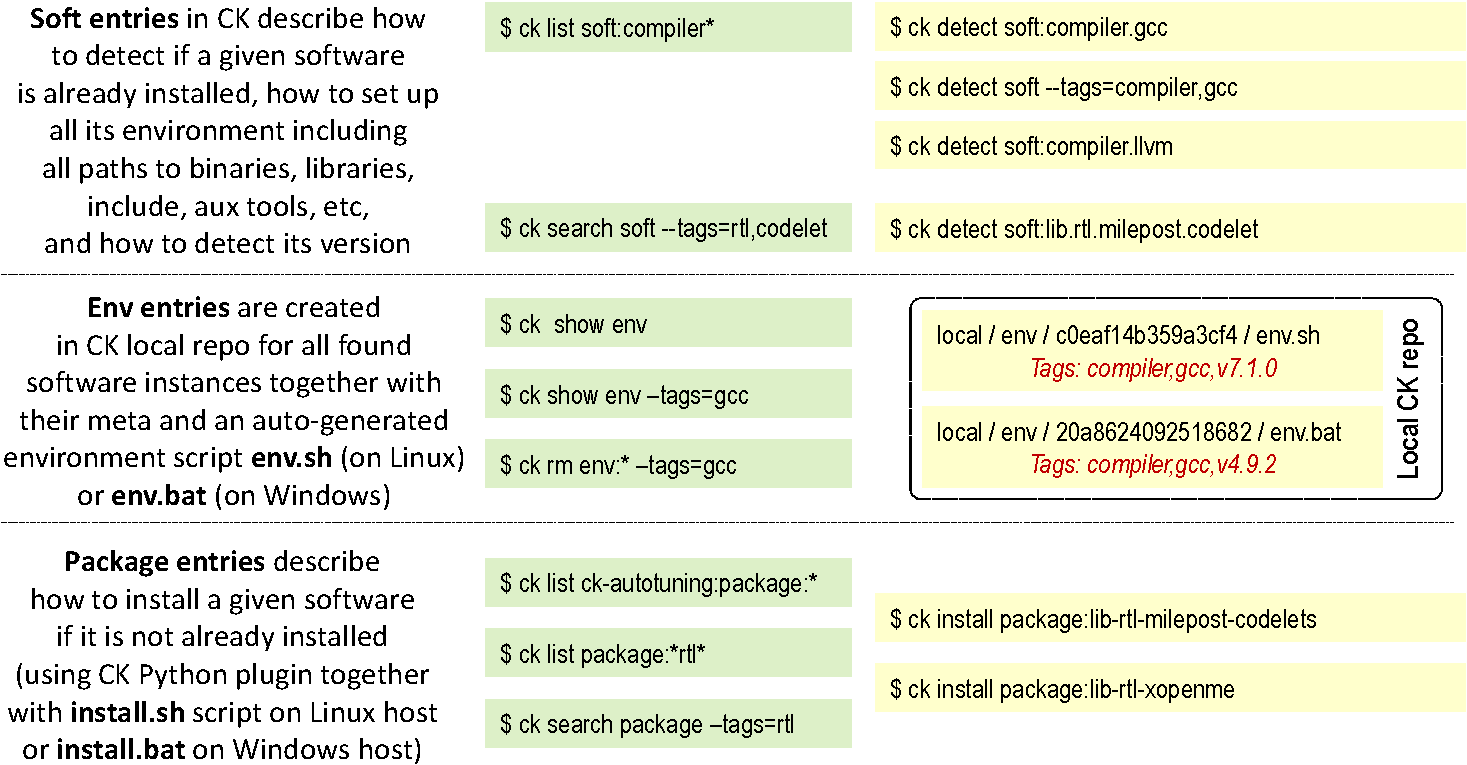
\includegraphics[width=5.6in]
      {ck-assets/01714ac89d5bd629-cropped.pdf} %CK_URL={01714ac89d5bd629-cropped.pdf}
     \caption{
   CK modules implementing portable package manager with JSON API to enable cross-platform CK workflows.
   The community shares CK entries with Python scripts and JSON meta information via Git repositories
   to describe how to detect, build and install any software. This approach also simplify
   co-existence of multiple versions of the same tool.
     }
     \label{fig:portable-package-manager}
   \end{figure*}
   %%%%%%%%%%%%%%%%%%%%%%%%%%%%%%%%%%%%%%%%%%%%%%%%%%%%%%%%%%%%%%%%%%%%%%%%%%%%%%%%%%%%%%%%%

Such approach extends the concept of package managers including
Spack~\cite{Gamblin:2015:SPM:2807591.2807623} and EasyBuild~\cite{DBLP:conf/sc/HosteTGW12}
by integrating them directly with experimental CK workflows while using unified CK API,
supporting any OS and platform, and allowing the community to gradually extend existing
detection or installation procedures via CK Python scripts and CK meta data.

Note that this CK approach encourages reuse of all such existing CK modules
from shared CK repositories rather then writing numerous ad-hoc scripts.
%
It should indeed be possible to substitute most of ad-hoc scripts
from public research projects (Figure~\ref{fig:convert-to-ck})
with just a few above modules and entries (Figure~\ref{fig:ck-repo}),
and then collaboratively extend them, thus dramatically improving research productivity.
%
For this reason, we keep track of all publicly shared modules and their repositories
in this \href{https://github.com/ctuning/ck/wiki/Shared-modules}{wiki page}.
%
The user will just need to add/update a \textit{.ckr.json} file
in the root directory of a given CK repository to describe a dependency
on other existing CK repositories with required modules or entries.
%
Since it is possible to uniquely reference any CK entry by two Unique IDs
(\textit{module UID:object UID}), we also plan to develop a simple web service
to automatically index and discover all modules similar to DOI.


   %%%%%%%%%%%%%%%%%%%%%%%%%%%%%%%%%%%%%%%%%%%%%%%%%%%%%%%%%%%%%%%%%%%%%%%%%%%%%%%%%%%%%%%%%
   %CK={"action":"prepare_for_latex", "cid":"slide:678dbc30be21a7ab", "file":"57ab625c176c52ad-cropped.pdf", "path":"ck-assets", "ck_image":"yes", "ck_image_width":400}
   \begin{figure}[htbp]
     \centering
      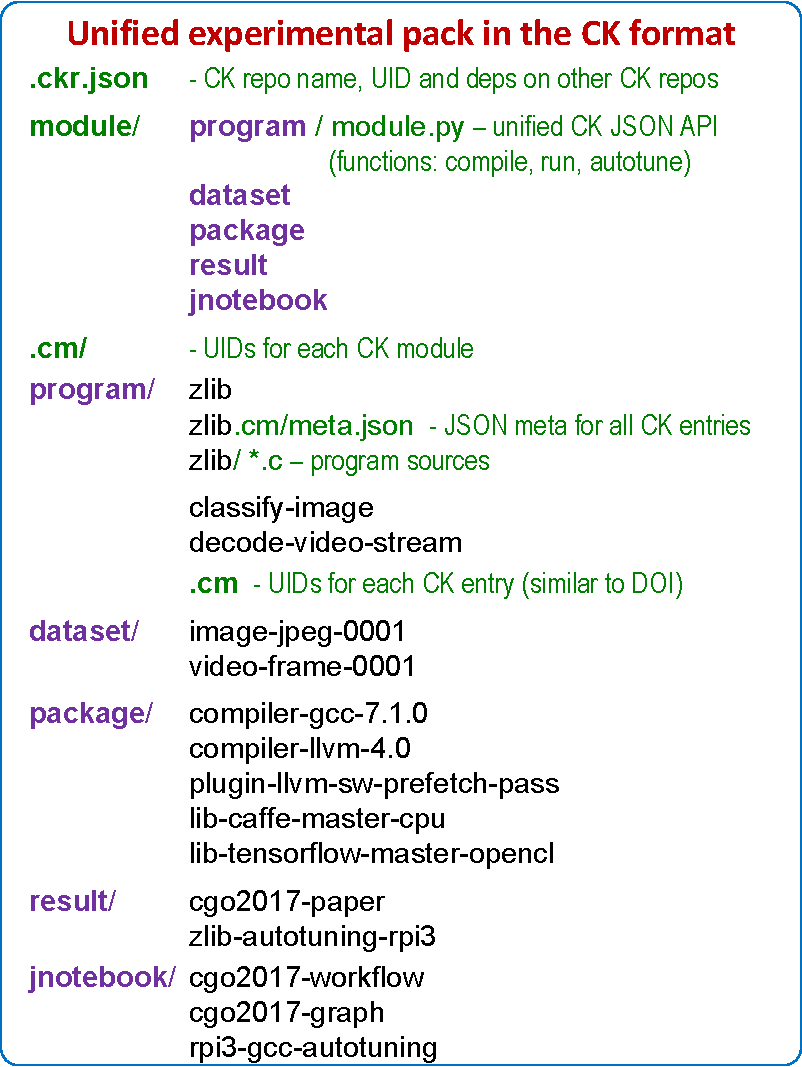
\includegraphics[width=3.4in]
      {ck-assets/57ab625c176c52ad-cropped.pdf} %CK_URL={57ab625c176c52ad-cropped.pdf}
     \caption{
        Typical experiment pack with reusable and discoverable components 
        shared in the CK format with two level directory structure (module and data).
     }
     \label{fig:ck-repo}
   \end{figure}
   %%%%%%%%%%%%%%%%%%%%%%%%%%%%%%%%%%%%%%%%%%%%%%%%%%%%%%%%%%%%%%%%%%%%%%%%%%%%%%%%%%%%%%%%%

The open, file-based format of CK repositories allows researchers
to continue editing entries and their meta directly using their favourite editors.
%
It also simplifies exchange of these entries using Git repositories, zip archives, Docker images 
and any other popular tool.
%
At the same time, schema-free and human readable Python dictionaries
and JSON files helps users to collaboratively extend actions, API and meta information
while keeping backward compatibility.
%
Such approach should let the community to gradually and collaboratively convert and
cross-link all existing ad-hoc code and data into unified components
with extensible API and meta information.
%
This, in turn, allows users organize their own research while reusing existing artifacts,
building upon them, improving them and continuously contributing back to Collective Knowledge
similar to Wikipedia.

We also noticed that CK can help students reduce preparation time 
for Artifact Evaluation~\cite{ctuning-ae1} at conferences while automating preparation 
and validation of experiments  since all artifacts, workflows and repositories are immediatelly ready
to be shared, ported and plugged in to research workflows.

For example, the highest ranked artifact from
the CGO'17 article~\cite{Ainsworth:2017:SPI:3049832.3049865}
was implemented and shared using the CK framework~\cite{cgo17-artifact}.
%
That is why CK is now used and publicly extended by leading
companies~\cite{ck-date16},
universities~\cite{Ainsworth:2017:SPI:3049832.3049865}
and organizations~\cite{ck-acm} to encourage, support and simplify
technology transfer between academia and industry.
